\begin{figure*}[t]
\centering
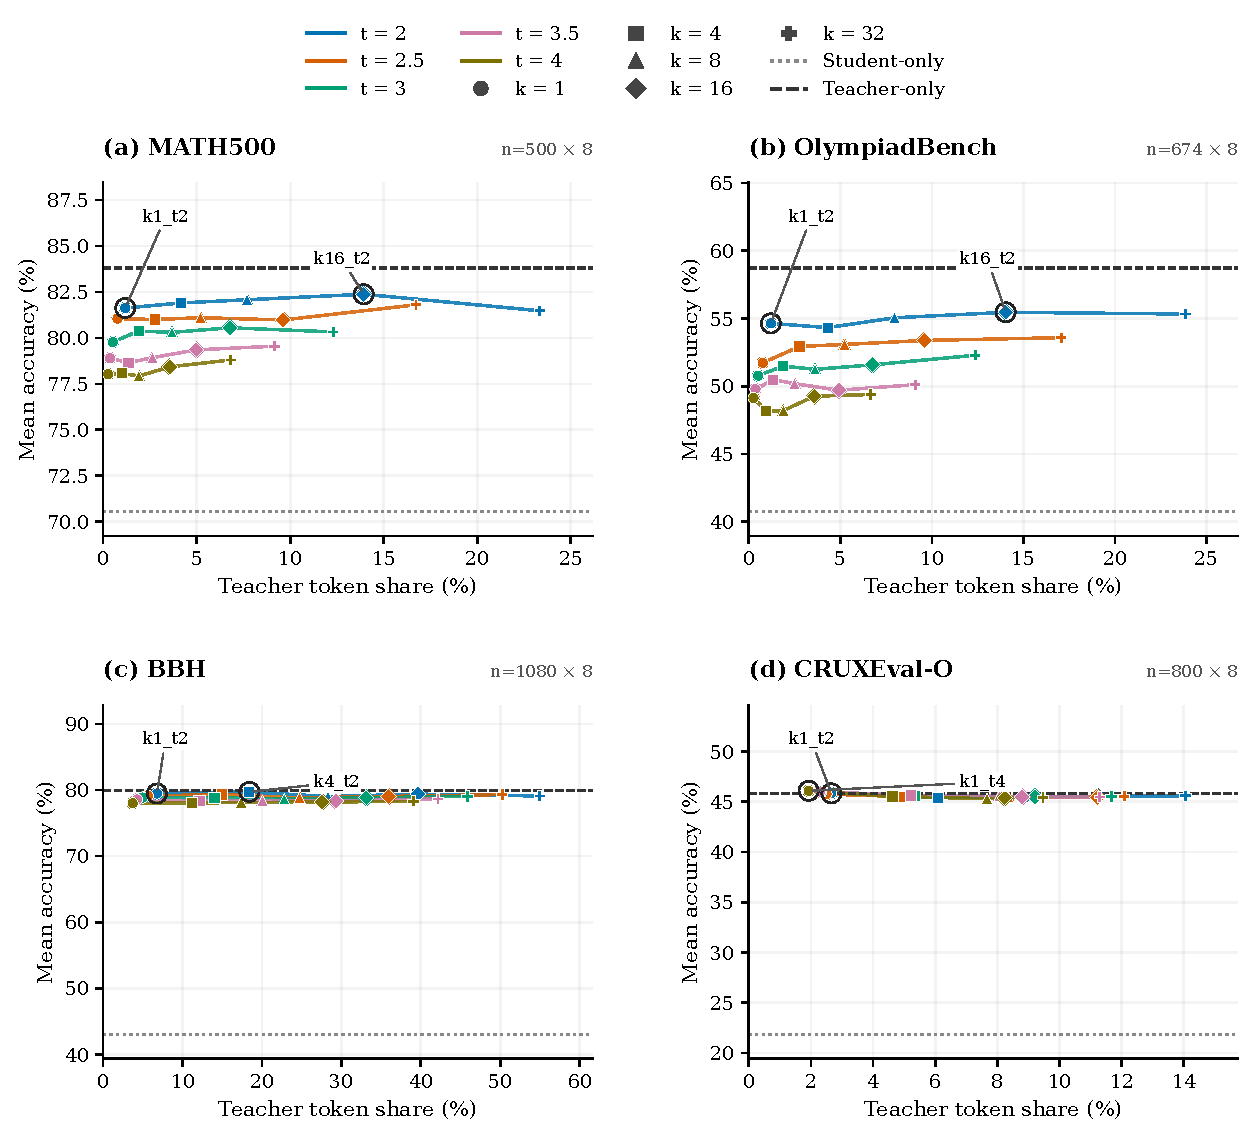
\includegraphics[width=\textwidth]{figures/main_grid_x8_20260920/accuracy_teacher_share_print_part1.pdf}
\caption{Mean accuracy versus Teacher token share for all 25 intervention configurations on each dataset. Colors denote thresholds and marker shapes denote k; lines connect points in increasing k, which need not increase token share. Horizontal lines show x8 Student-only and Teacher-only accuracy references, not their token-share coordinates (0\% and 100\%, respectively). Circled and annotated points are k1\_t2 and all configurations attaining the observed maximum accuracy. Axes are scaled independently across panels. Teacher token share is the ratio of total Teacher output tokens to total output tokens; it excludes prompt, discarded drafts and Teacher scoring overhead and is not a compute-cost or speedup measure. Part 1 of 2. All configurations and baselines use eight rollouts per question, with the same question counts within each dataset. Student: Qwen3-1.7B; Teacher: Qwen3-14B. Math/reasoning replicate 0 differs from later replicates in judge/extraction and timeout protocol; deployment concurrency also varied. Generation timeouts are counted as incorrect. Results are descriptive, with no confidence intervals or significance claims.}
\label{fig:accuracy-teacher-share-print-part1}
\end{figure*}

\begin{figure*}[t]
\centering
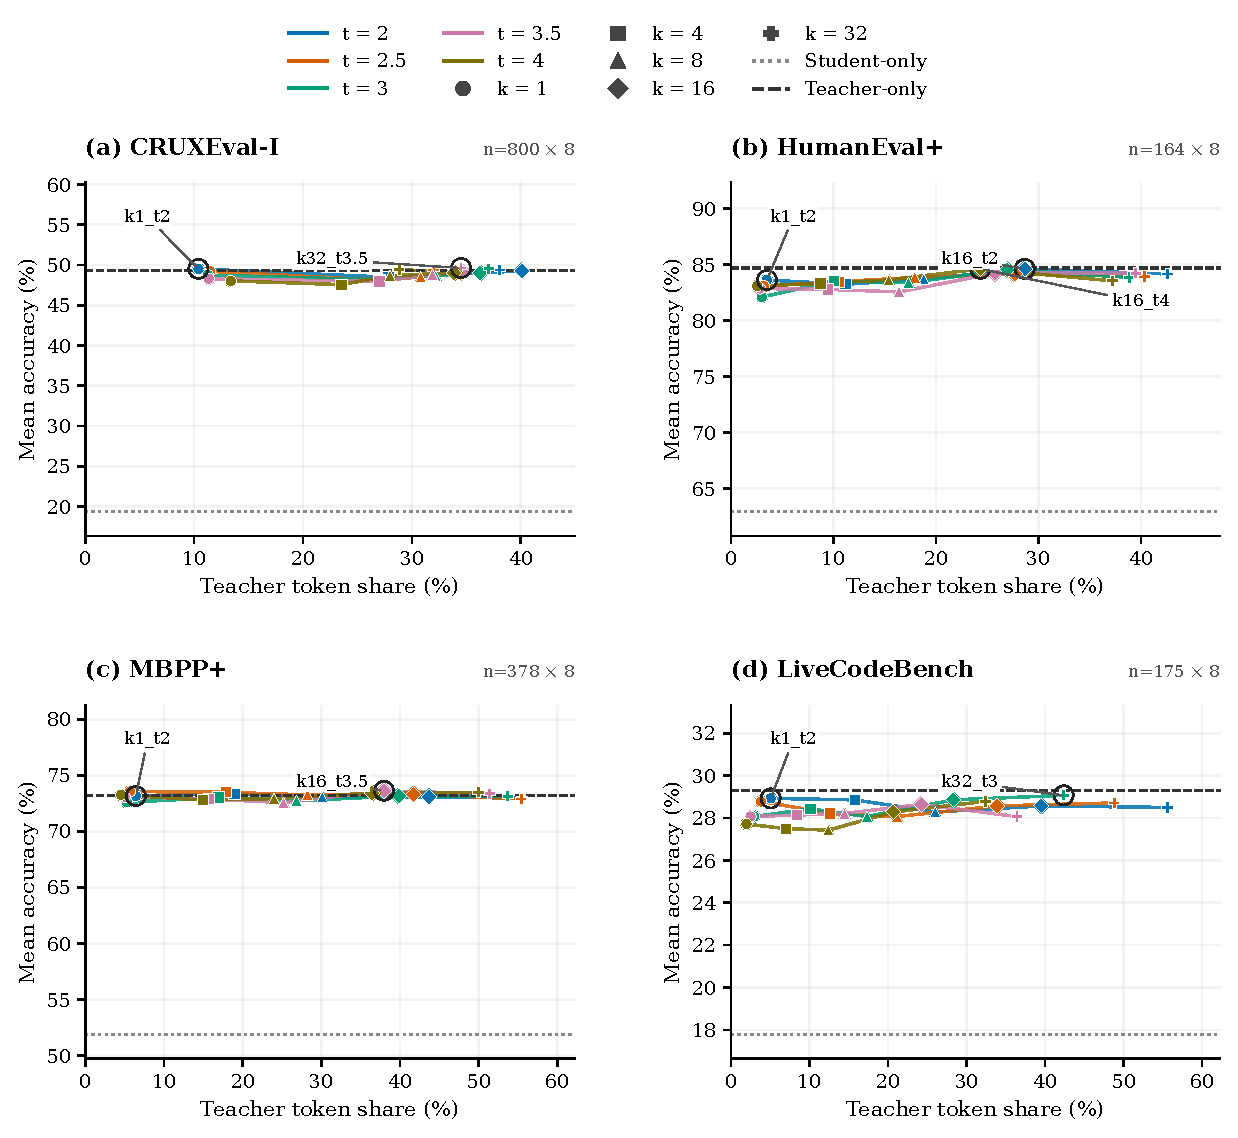
\includegraphics[width=\textwidth]{figures/main_grid_x8_20260920/accuracy_teacher_share_print_part2.pdf}
\caption{Mean accuracy versus Teacher token share for all 25 intervention configurations on each dataset. Colors denote thresholds and marker shapes denote k; lines connect points in increasing k, which need not increase token share. Horizontal lines show x8 Student-only and Teacher-only accuracy references, not their token-share coordinates (0\% and 100\%, respectively). Circled and annotated points are k1\_t2 and all configurations attaining the observed maximum accuracy. Axes are scaled independently across panels. Teacher token share is the ratio of total Teacher output tokens to total output tokens; it excludes prompt, discarded drafts and Teacher scoring overhead and is not a compute-cost or speedup measure. Part 2 of 2. All configurations and baselines use eight rollouts per question, with the same question counts within each dataset. Student: Qwen3-1.7B; Teacher: Qwen3-14B. Math/reasoning replicate 0 differs from later replicates in judge/extraction and timeout protocol; deployment concurrency also varied. Generation timeouts are counted as incorrect. Results are descriptive, with no confidence intervals or significance claims.}
\label{fig:accuracy-teacher-share-print-part2}
\end{figure*}

\begin{figure*}[t]
\centering
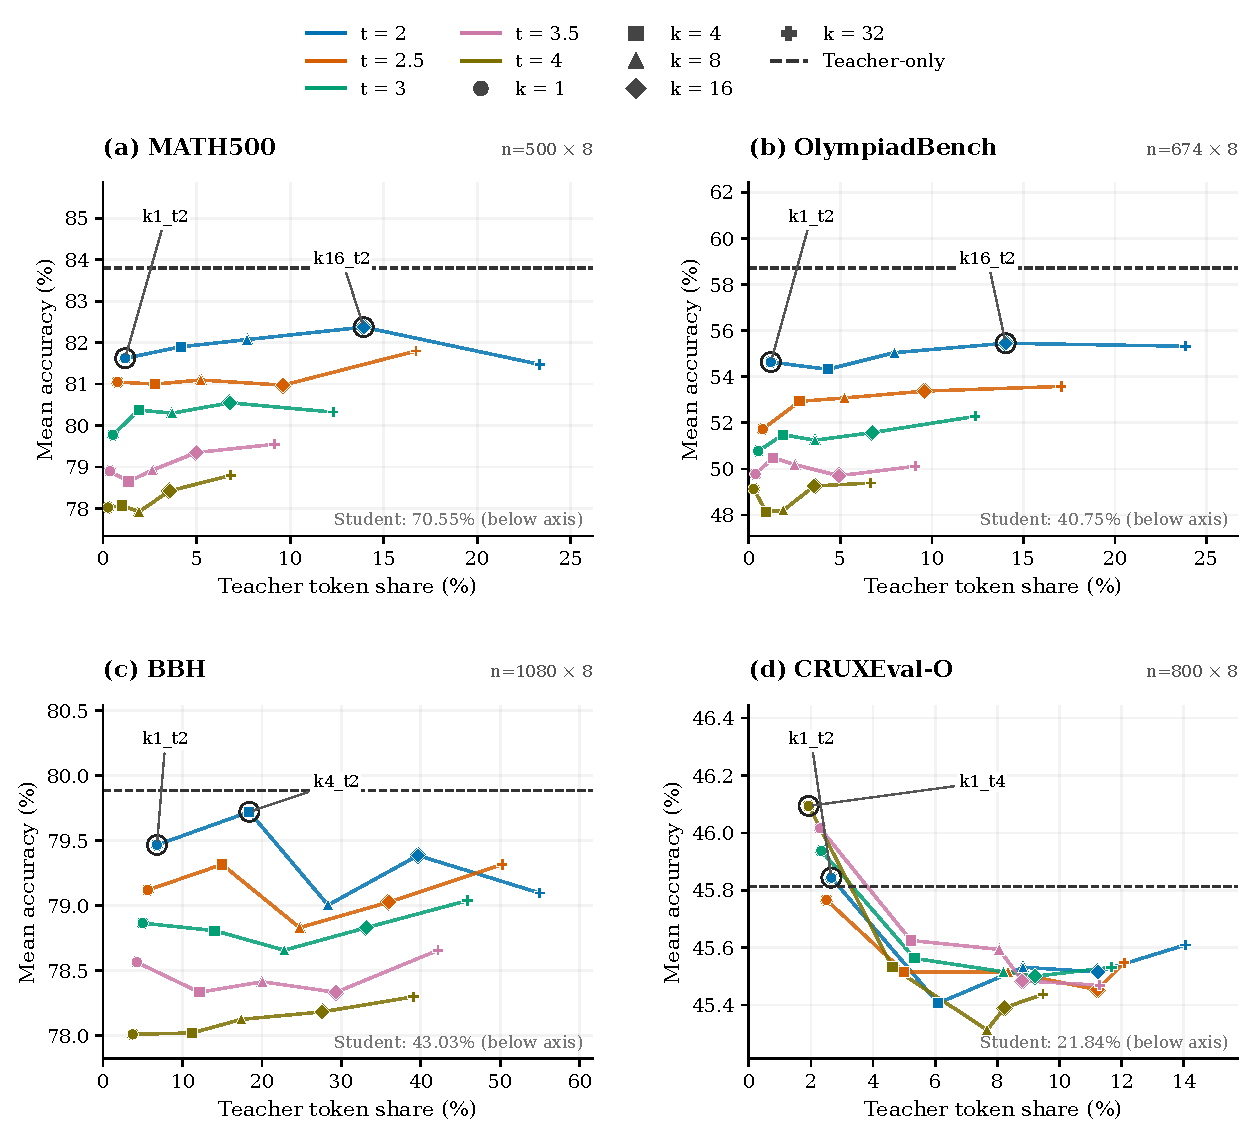
\includegraphics[width=\textwidth]{figures/main_grid_x8_20260920/accuracy_teacher_share_zoom_print_part1.pdf}
\caption{Detail view of the accuracy–Teacher token tradeoff, with independently zoomed vertical axes. Student-only accuracy lies below every panel and is stated numerically; Teacher-only is a horizontal reference. All data, color/marker encodings and selected annotations match the full-range figure. Small observed differences do not imply statistical significance. Part 1 of 2. All configurations and baselines use eight rollouts per question, with the same question counts within each dataset. Student: Qwen3-1.7B; Teacher: Qwen3-14B. Math/reasoning replicate 0 differs from later replicates in judge/extraction and timeout protocol; deployment concurrency also varied. Generation timeouts are counted as incorrect. Results are descriptive, with no confidence intervals or significance claims.}
\label{fig:accuracy-teacher-share-zoom-print-part1}
\end{figure*}

\begin{figure*}[t]
\centering
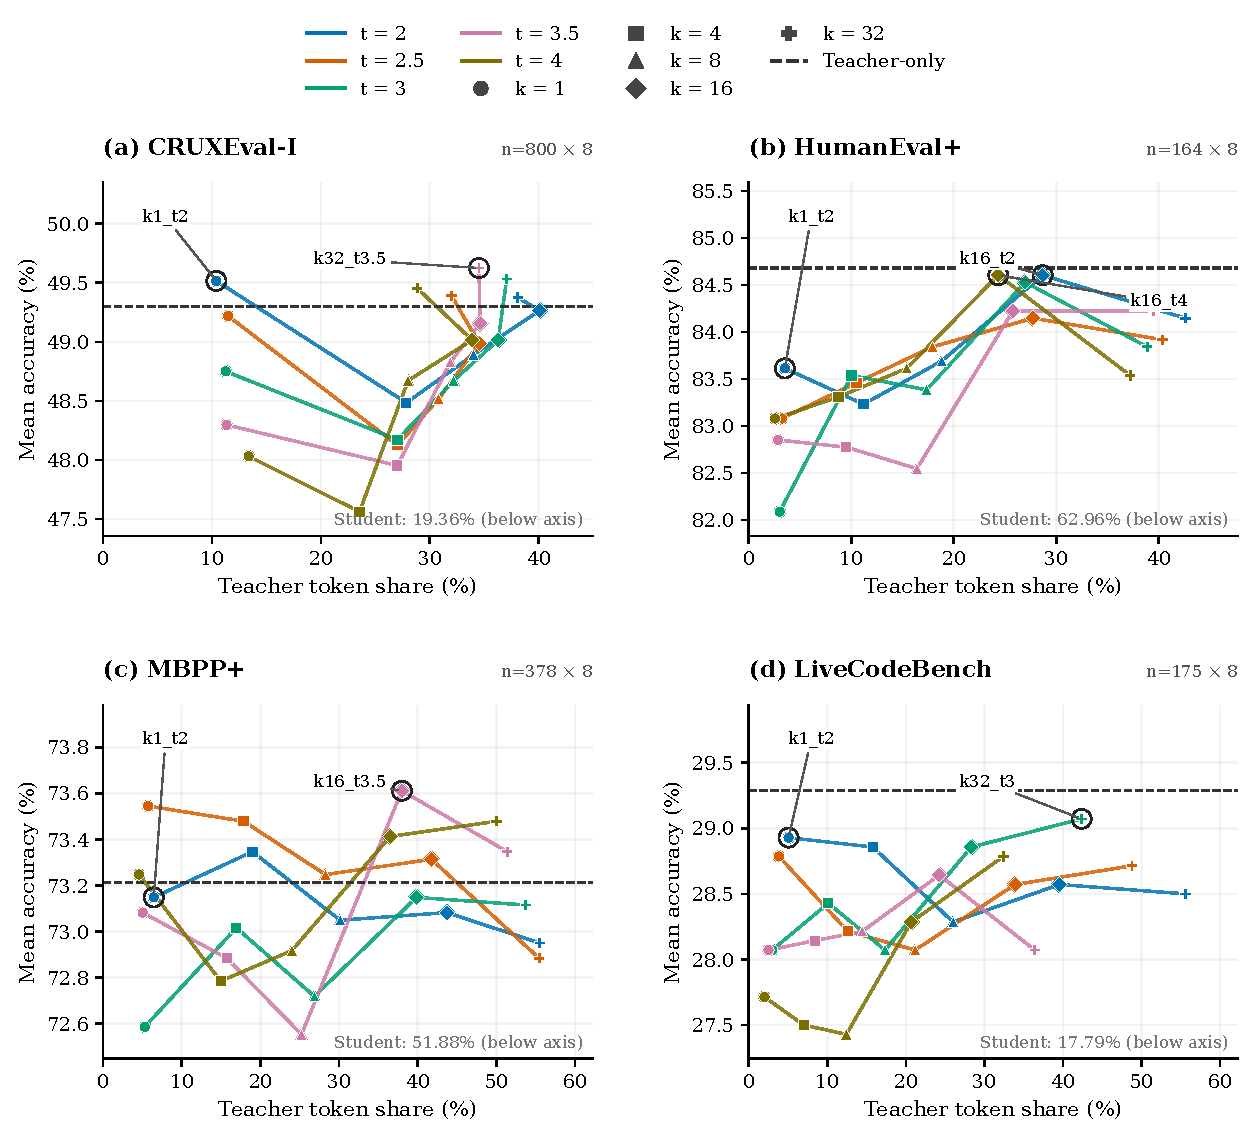
\includegraphics[width=\textwidth]{figures/main_grid_x8_20260920/accuracy_teacher_share_zoom_print_part2.pdf}
\caption{Detail view of the accuracy–Teacher token tradeoff, with independently zoomed vertical axes. Student-only accuracy lies below every panel and is stated numerically; Teacher-only is a horizontal reference. All data, color/marker encodings and selected annotations match the full-range figure. Small observed differences do not imply statistical significance. Part 2 of 2. All configurations and baselines use eight rollouts per question, with the same question counts within each dataset. Student: Qwen3-1.7B; Teacher: Qwen3-14B. Math/reasoning replicate 0 differs from later replicates in judge/extraction and timeout protocol; deployment concurrency also varied. Generation timeouts are counted as incorrect. Results are descriptive, with no confidence intervals or significance claims.}
\label{fig:accuracy-teacher-share-zoom-print-part2}
\end{figure*}

\begin{figure*}[t]
\centering
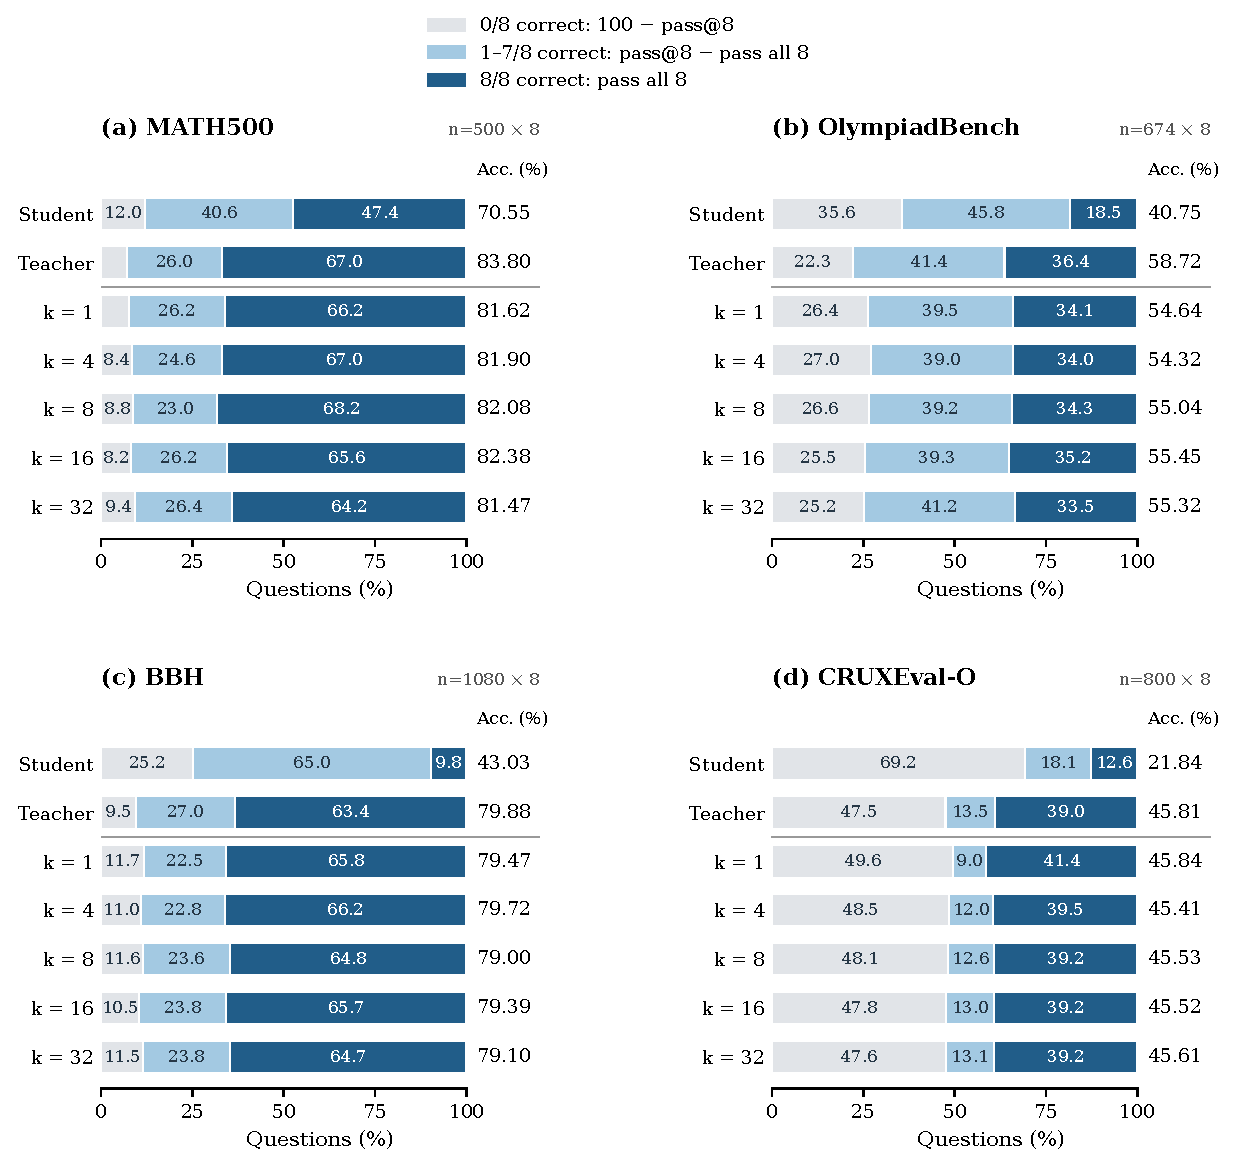
\includegraphics[width=\textwidth]{figures/main_grid_x8_20260920/stability_t2_print_part1.pdf}
\caption{Per-question outcomes over eight rollouts for Student-only, Teacher-only and all five k values at threshold 2. Gray denotes zero correct rollouts (100 minus pass@8); light blue denotes one to seven correct rollouts (pass@8 minus pass all 8); dark blue denotes eight correct rollouts (pass all 8). Bars sum to 100\%; right-hand values give mean accuracy over all outputs. Segment labels are percentages and are omitted below 8\% for readability. The subset is fixed by threshold, not selected by each dataset’s best accuracy. Part 1 of 2. All configurations and baselines use eight rollouts per question, with the same question counts within each dataset. Student: Qwen3-1.7B; Teacher: Qwen3-14B. Math/reasoning replicate 0 differs from later replicates in judge/extraction and timeout protocol; deployment concurrency also varied. Generation timeouts are counted as incorrect. Results are descriptive, with no confidence intervals or significance claims.}
\label{fig:stability-t2-print-part1}
\end{figure*}

\begin{figure*}[t]
\centering
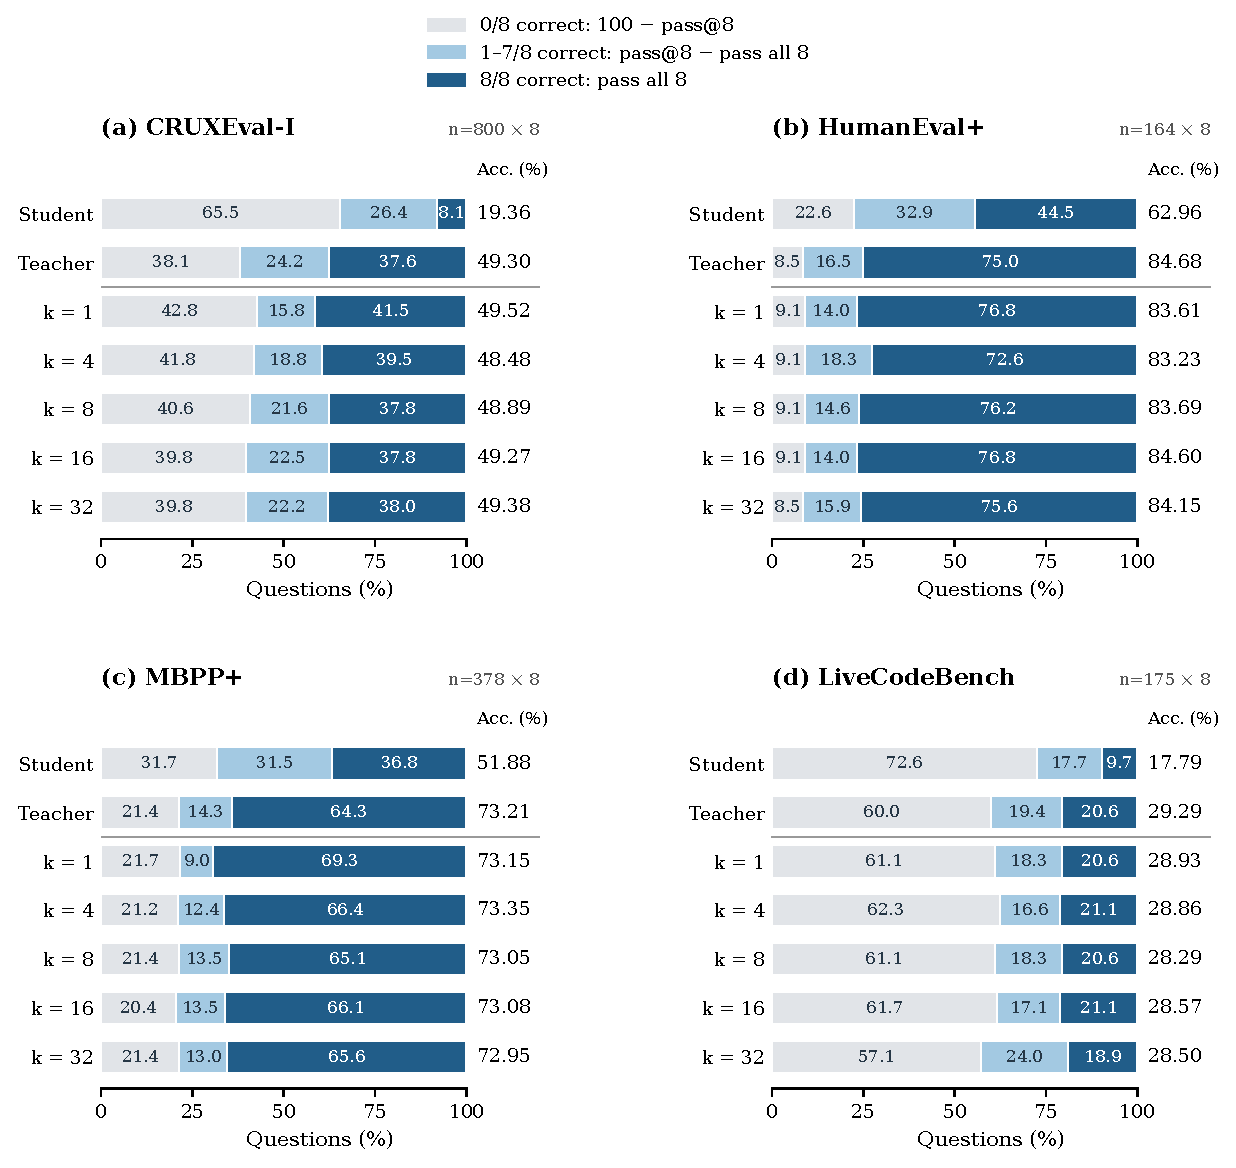
\includegraphics[width=\textwidth]{figures/main_grid_x8_20260920/stability_t2_print_part2.pdf}
\caption{Per-question outcomes over eight rollouts for Student-only, Teacher-only and all five k values at threshold 2. Gray denotes zero correct rollouts (100 minus pass@8); light blue denotes one to seven correct rollouts (pass@8 minus pass all 8); dark blue denotes eight correct rollouts (pass all 8). Bars sum to 100\%; right-hand values give mean accuracy over all outputs. Segment labels are percentages and are omitted below 8\% for readability. The subset is fixed by threshold, not selected by each dataset’s best accuracy. Part 2 of 2. All configurations and baselines use eight rollouts per question, with the same question counts within each dataset. Student: Qwen3-1.7B; Teacher: Qwen3-14B. Math/reasoning replicate 0 differs from later replicates in judge/extraction and timeout protocol; deployment concurrency also varied. Generation timeouts are counted as incorrect. Results are descriptive, with no confidence intervals or significance claims.}
\label{fig:stability-t2-print-part2}
\end{figure*}

\begin{figure*}[t]
\centering
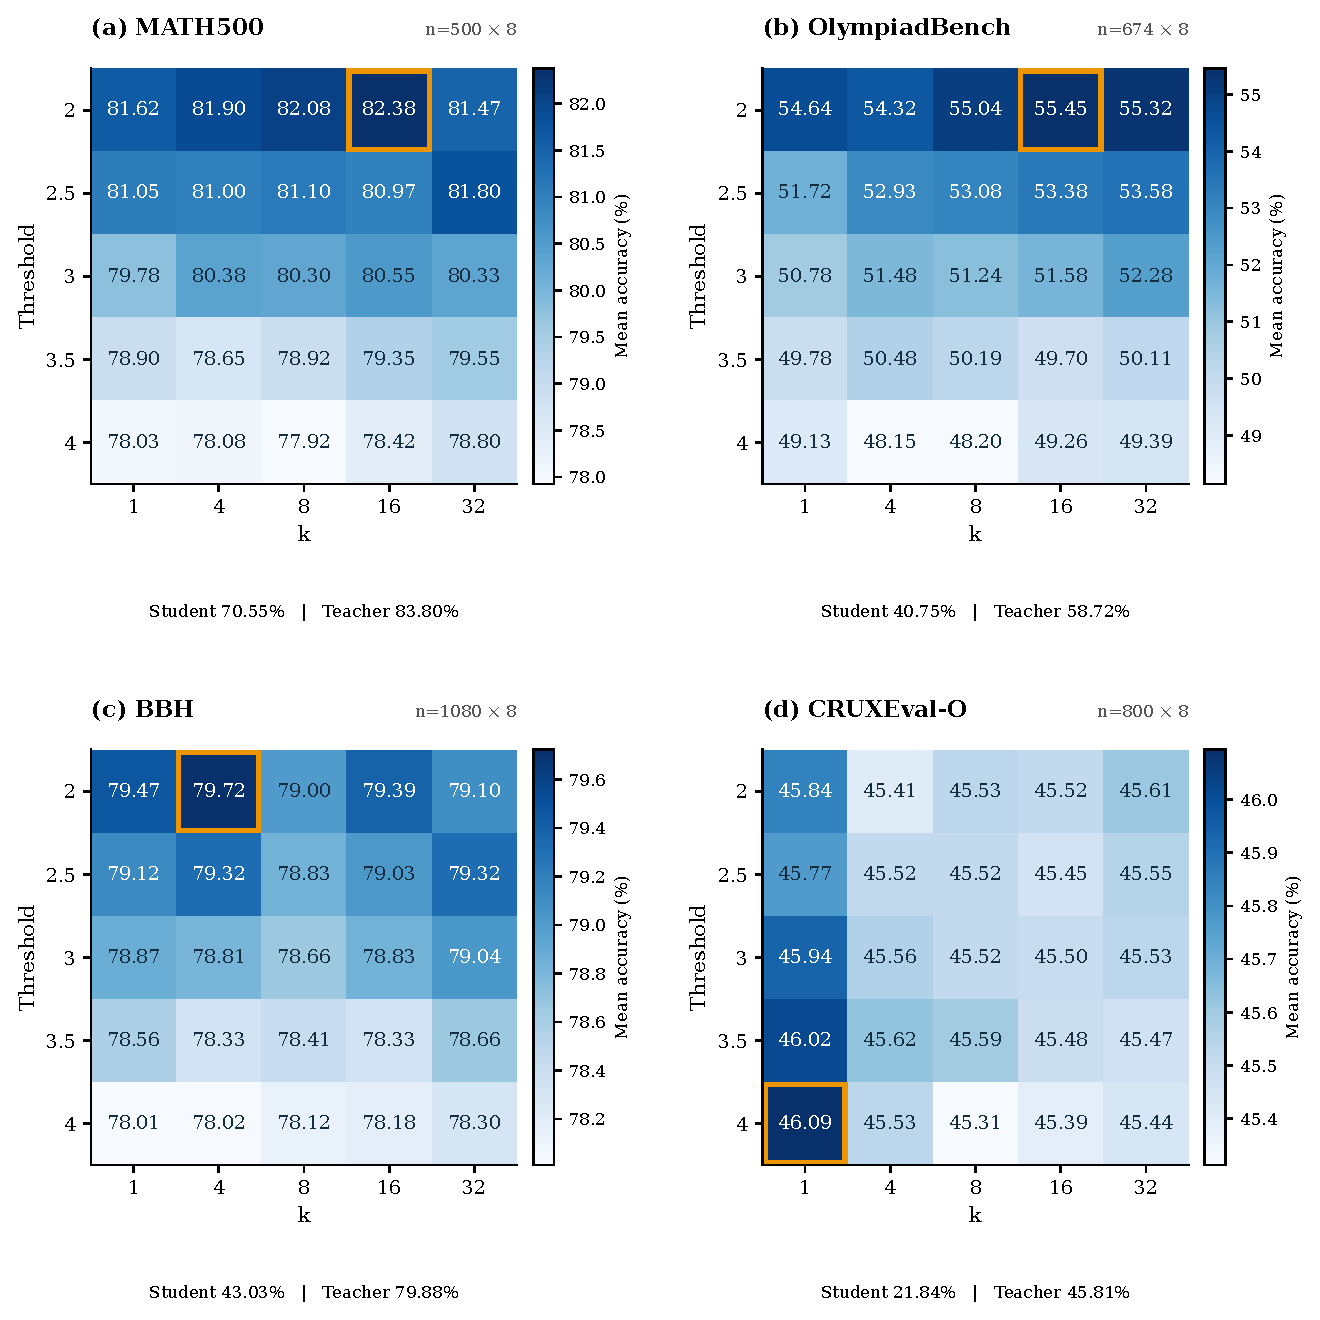
\includegraphics[width=\textwidth]{figures/main_grid_x8_20260920/accuracy_heatmap_print_part1.pdf}
\caption{Mean accuracy (\%) across the full threshold-by-k grid. Each panel uses its own labeled color scale; color intensity is not comparable across datasets. Orange outlines mark every maximum computed before rounding, including ties. Student-only and Teacher-only x8 accuracies appear beneath each panel. Part 1 of 2. All configurations and baselines use eight rollouts per question, with the same question counts within each dataset. Student: Qwen3-1.7B; Teacher: Qwen3-14B. Math/reasoning replicate 0 differs from later replicates in judge/extraction and timeout protocol; deployment concurrency also varied. Generation timeouts are counted as incorrect. Results are descriptive, with no confidence intervals or significance claims.}
\label{fig:accuracy-heatmap-print-part1}
\end{figure*}

\begin{figure*}[t]
\centering
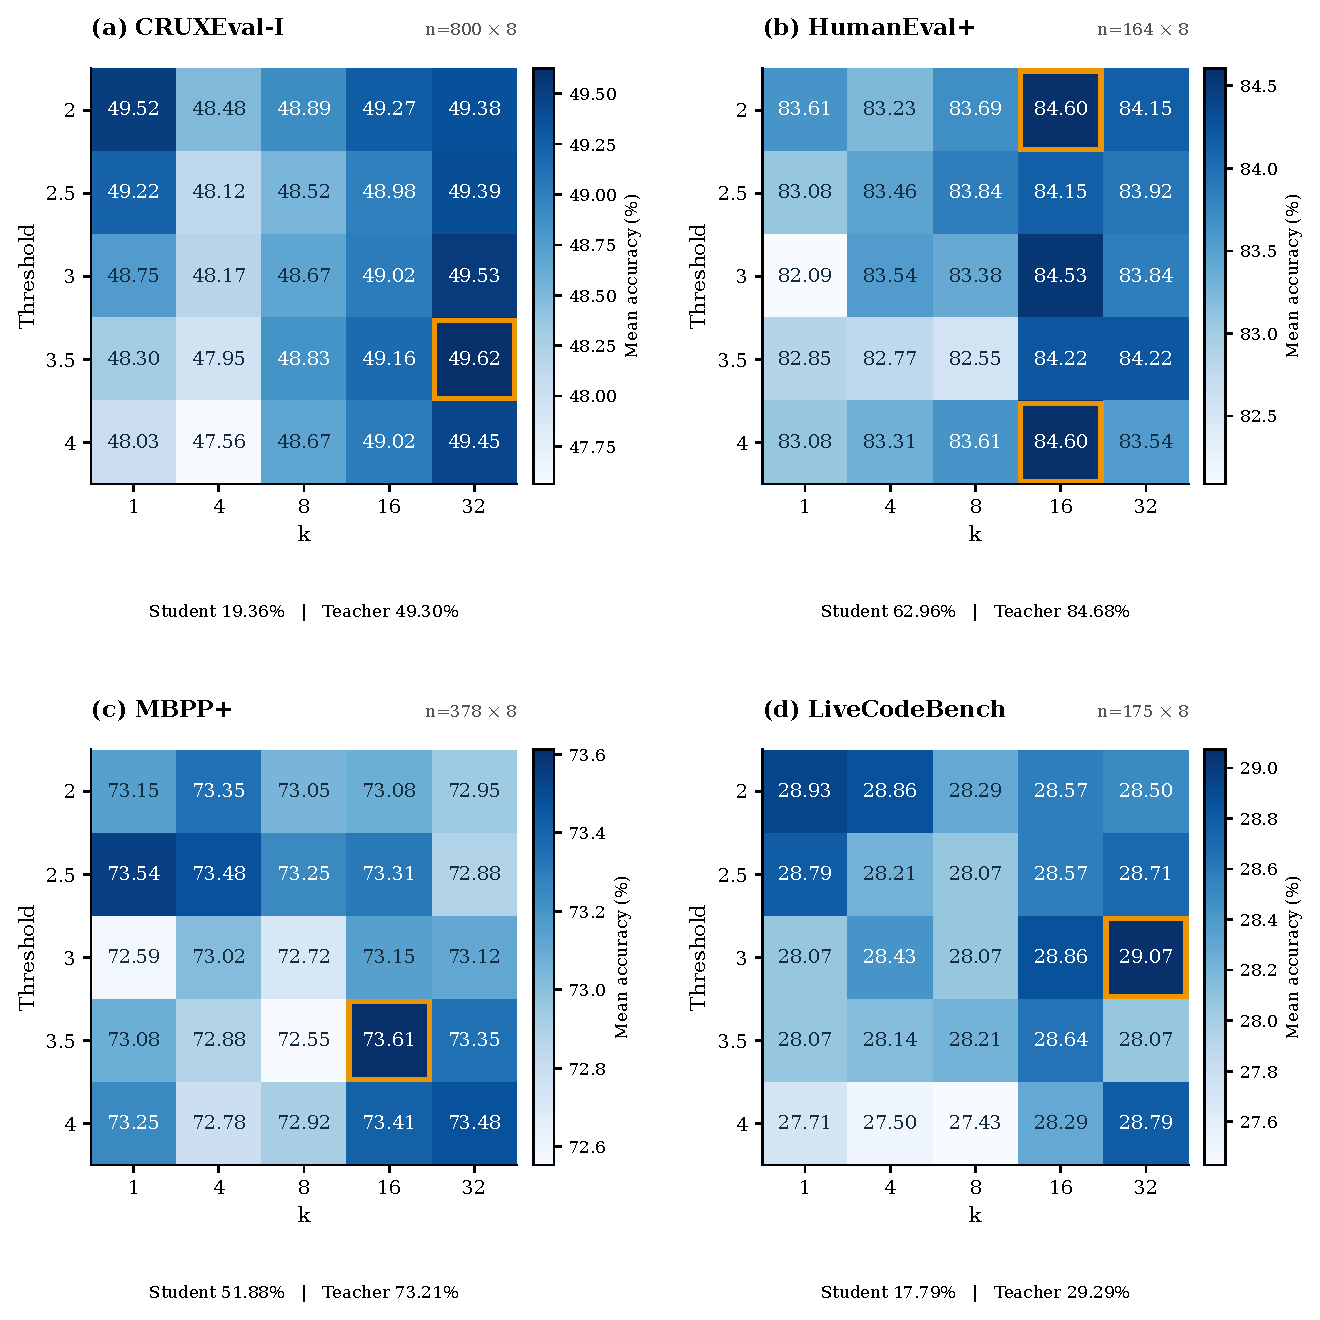
\includegraphics[width=\textwidth]{figures/main_grid_x8_20260920/accuracy_heatmap_print_part2.pdf}
\caption{Mean accuracy (\%) across the full threshold-by-k grid. Each panel uses its own labeled color scale; color intensity is not comparable across datasets. Orange outlines mark every maximum computed before rounding, including ties. Student-only and Teacher-only x8 accuracies appear beneath each panel. Part 2 of 2. All configurations and baselines use eight rollouts per question, with the same question counts within each dataset. Student: Qwen3-1.7B; Teacher: Qwen3-14B. Math/reasoning replicate 0 differs from later replicates in judge/extraction and timeout protocol; deployment concurrency also varied. Generation timeouts are counted as incorrect. Results are descriptive, with no confidence intervals or significance claims.}
\label{fig:accuracy-heatmap-print-part2}
\end{figure*}

\begin{figure*}[t]
\centering
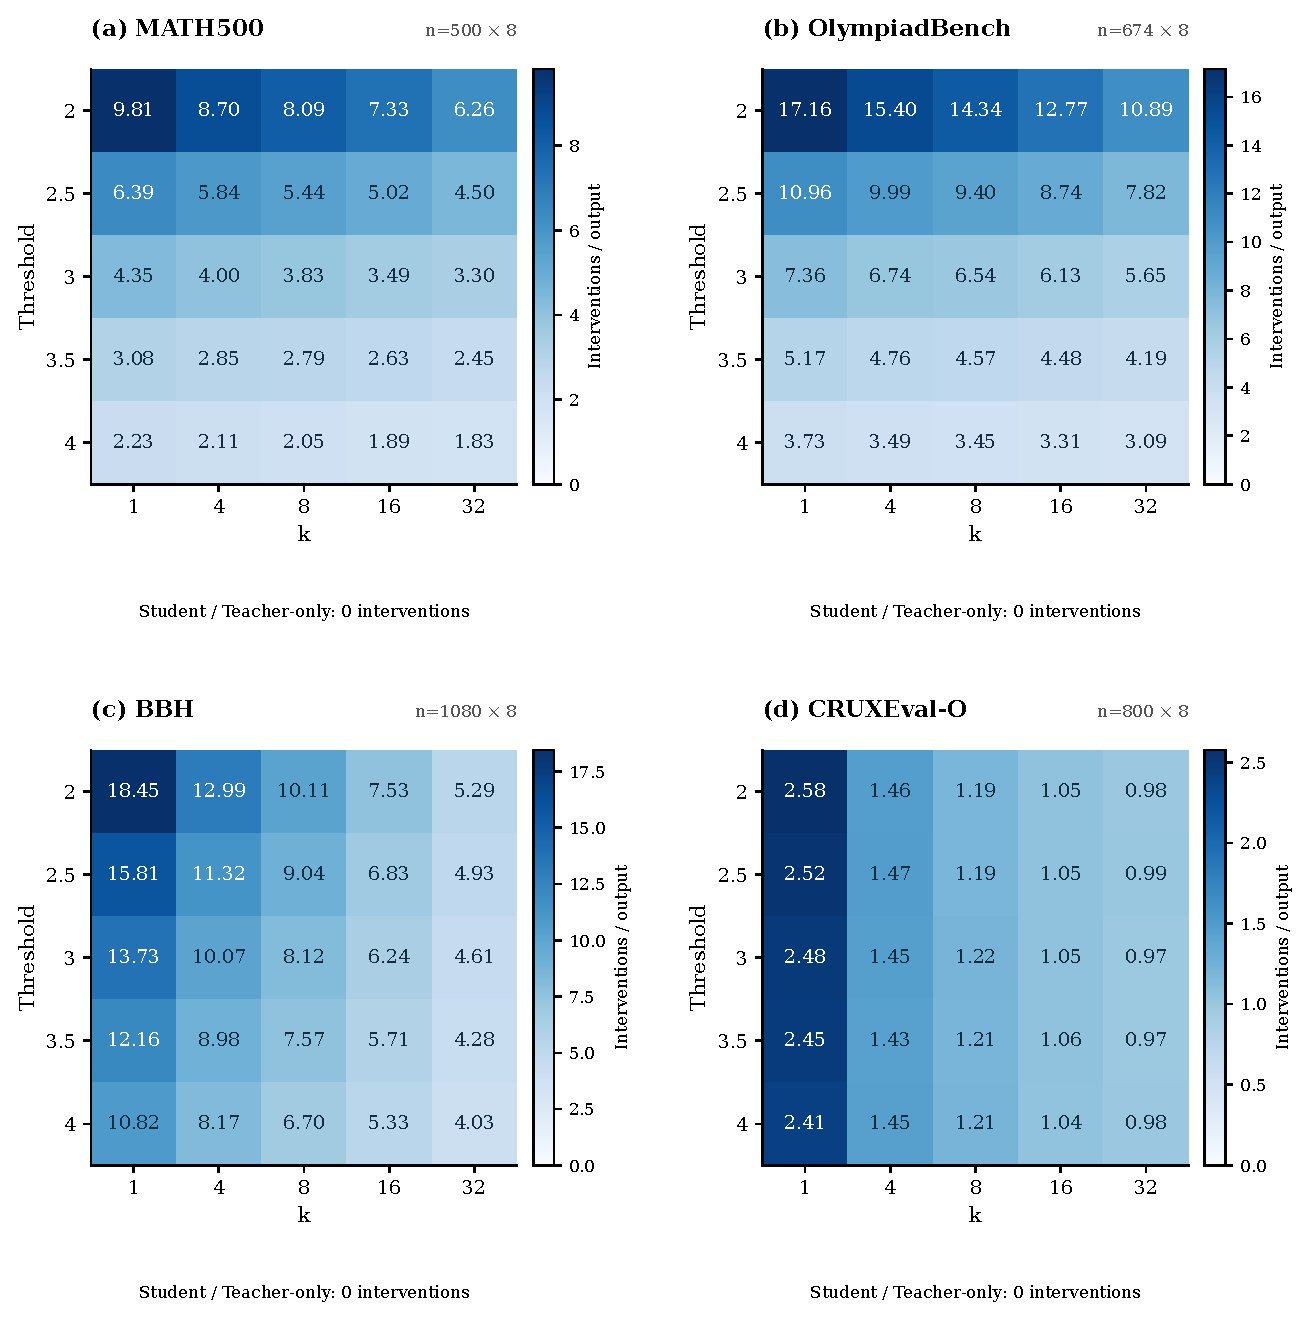
\includegraphics[width=\textwidth]{figures/main_grid_x8_20260920/interventions_heatmap_print_part1.pdf}
\caption{Mean number of Teacher interventions per generated output across the threshold-by-k grid, including zero-intervention and timeout samples. Both standalone baselines have zero interventions. Each panel has its own labeled color scale. Dataset ordering follows the accuracy heatmap. Part 1 of 2. All configurations and baselines use eight rollouts per question, with the same question counts within each dataset. Student: Qwen3-1.7B; Teacher: Qwen3-14B. Math/reasoning replicate 0 differs from later replicates in judge/extraction and timeout protocol; deployment concurrency also varied. Generation timeouts are counted as incorrect. Results are descriptive, with no confidence intervals or significance claims.}
\label{fig:interventions-heatmap-print-part1}
\end{figure*}

\begin{figure*}[t]
\centering
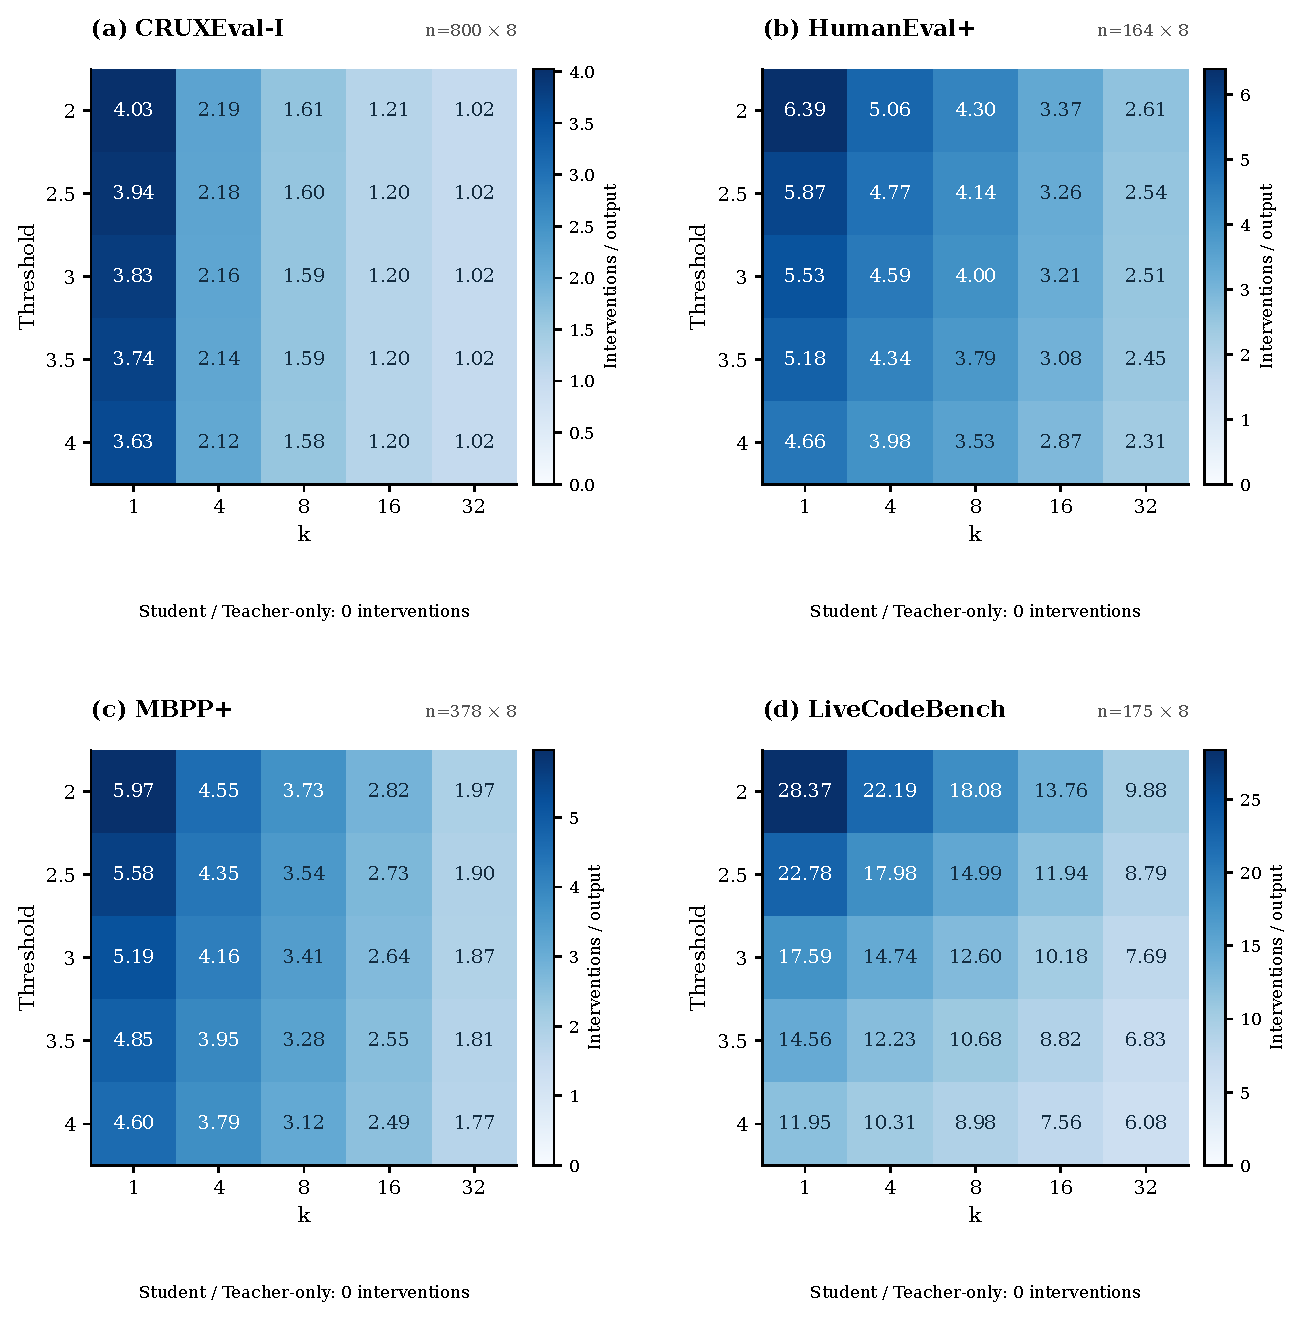
\includegraphics[width=\textwidth]{figures/main_grid_x8_20260920/interventions_heatmap_print_part2.pdf}
\caption{Mean number of Teacher interventions per generated output across the threshold-by-k grid, including zero-intervention and timeout samples. Both standalone baselines have zero interventions. Each panel has its own labeled color scale. Dataset ordering follows the accuracy heatmap. Part 2 of 2. All configurations and baselines use eight rollouts per question, with the same question counts within each dataset. Student: Qwen3-1.7B; Teacher: Qwen3-14B. Math/reasoning replicate 0 differs from later replicates in judge/extraction and timeout protocol; deployment concurrency also varied. Generation timeouts are counted as incorrect. Results are descriptive, with no confidence intervals or significance claims.}
\label{fig:interventions-heatmap-print-part2}
\end{figure*}

\begin{figure*}[t]
\centering
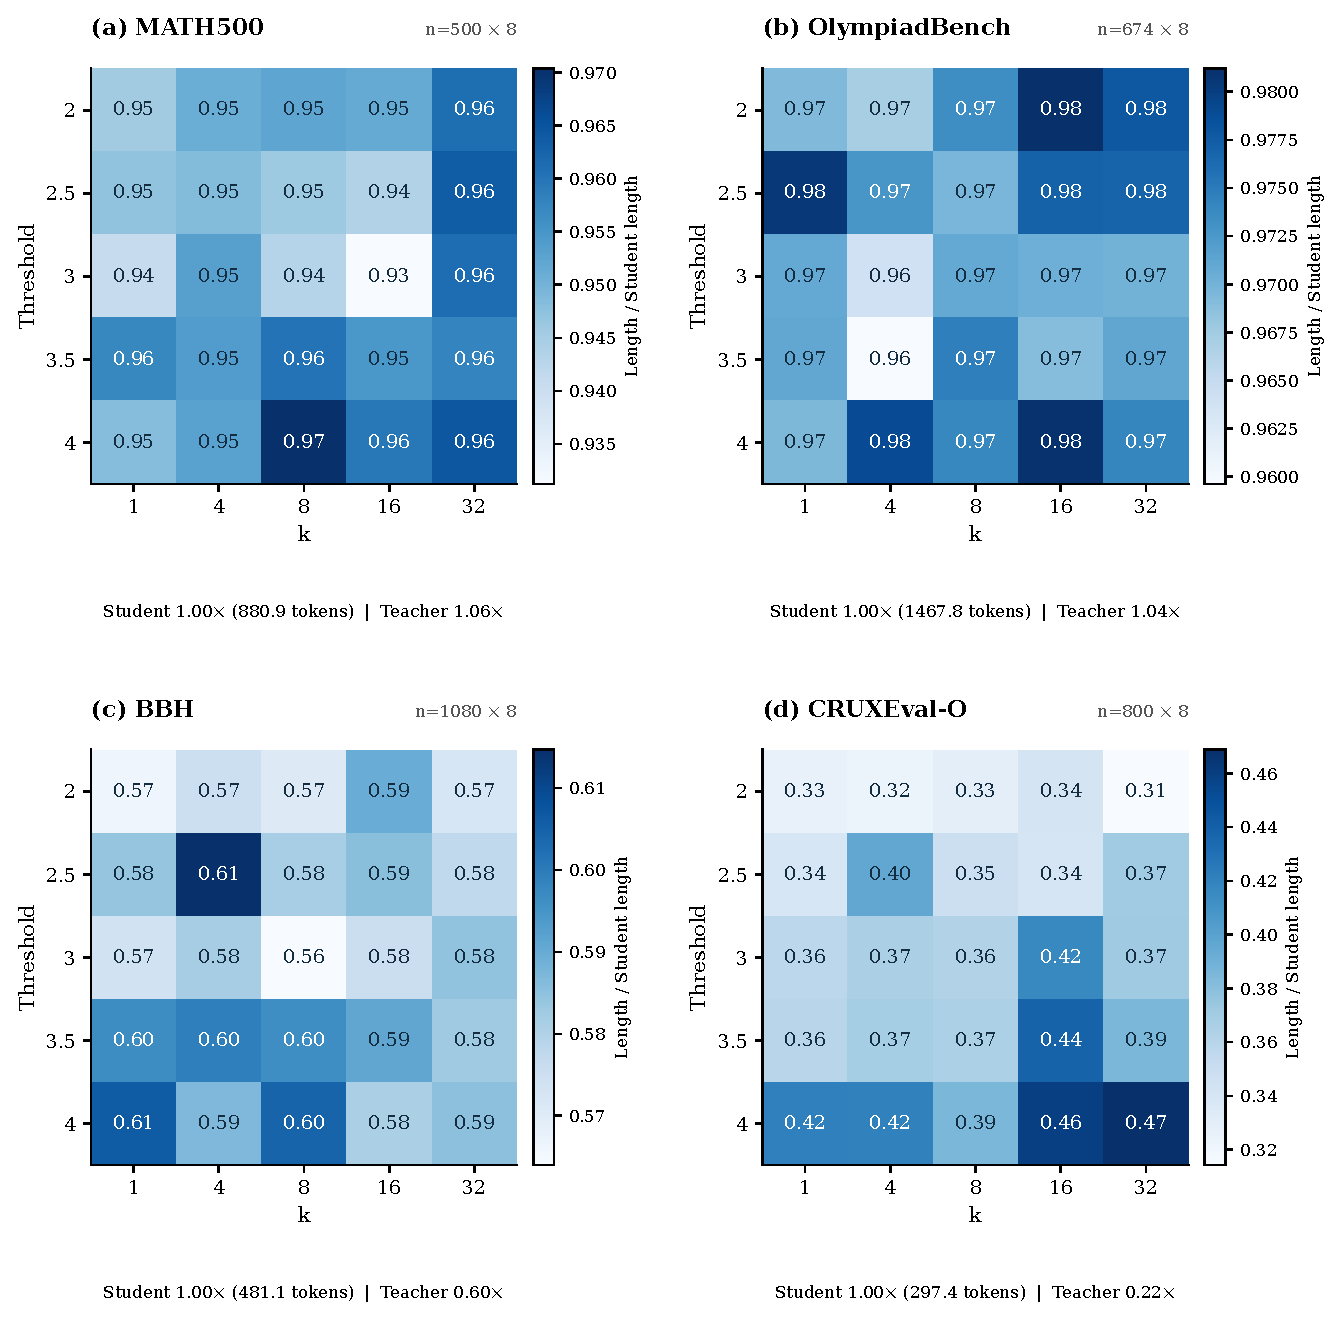
\includegraphics[width=\textwidth]{figures/main_grid_x8_20260920/length_ratio_heatmap_print_part1.pdf}
\caption{Mean output length divided by the same dataset’s x8 Student-only mean output length. Ratios are computed from unrounded totals and include timeout samples; values below one indicate shorter outputs. Student baseline token lengths and Teacher/Student length ratios appear beneath each panel. Each panel has its own labeled color scale, so compare printed ratios across datasets. Part 1 of 2. All configurations and baselines use eight rollouts per question, with the same question counts within each dataset. Student: Qwen3-1.7B; Teacher: Qwen3-14B. Math/reasoning replicate 0 differs from later replicates in judge/extraction and timeout protocol; deployment concurrency also varied. Generation timeouts are counted as incorrect. Results are descriptive, with no confidence intervals or significance claims.}
\label{fig:length-ratio-heatmap-print-part1}
\end{figure*}

\begin{figure*}[t]
\centering
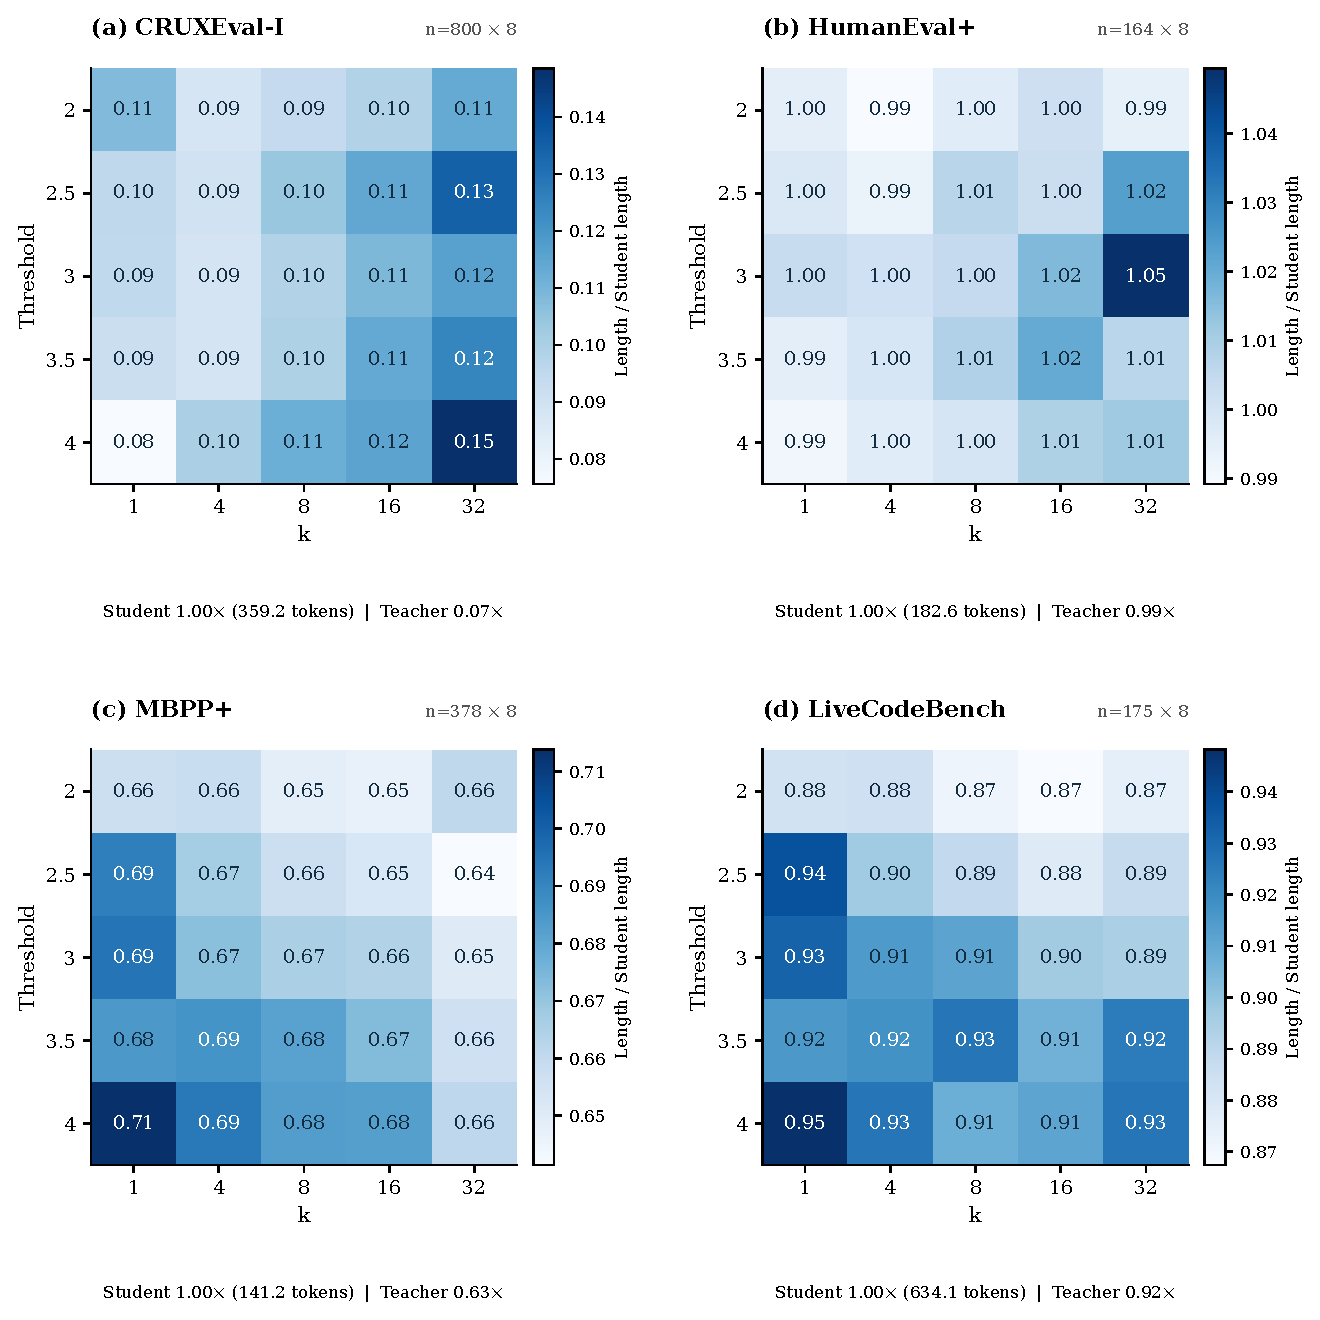
\includegraphics[width=\textwidth]{figures/main_grid_x8_20260920/length_ratio_heatmap_print_part2.pdf}
\caption{Mean output length divided by the same dataset’s x8 Student-only mean output length. Ratios are computed from unrounded totals and include timeout samples; values below one indicate shorter outputs. Student baseline token lengths and Teacher/Student length ratios appear beneath each panel. Each panel has its own labeled color scale, so compare printed ratios across datasets. Part 2 of 2. All configurations and baselines use eight rollouts per question, with the same question counts within each dataset. Student: Qwen3-1.7B; Teacher: Qwen3-14B. Math/reasoning replicate 0 differs from later replicates in judge/extraction and timeout protocol; deployment concurrency also varied. Generation timeouts are counted as incorrect. Results are descriptive, with no confidence intervals or significance claims.}
\label{fig:length-ratio-heatmap-print-part2}
\end{figure*}
